\section{Results}

We can use the uniqueness measure to understand the rate at which new ideas arrive. As we gather more and more ideas in the course of an experiment, we expect that we will see fewer ideas that are not already in our idea pool. Figure FIG shows the cumulative count of ideas as a function of the number of instances gathered in the experiment. To smooth the plot, the order in which instances were received was shuffled 100 times, and the mean of the cumulative unique idea count was taken at each step.

\begin{figure}[h!]
    \centering
    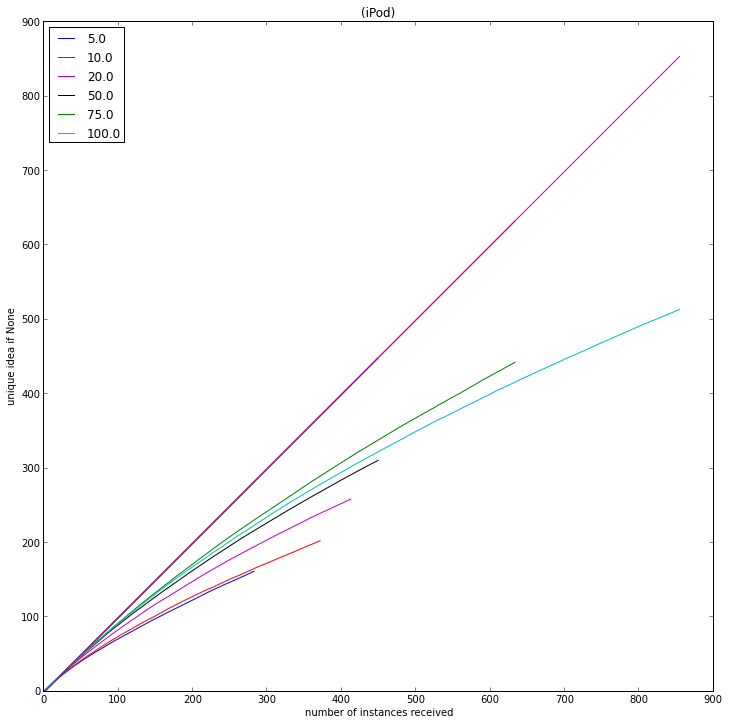
\includegraphics[width=0.9\columnwidth]{ideas_over_time}
    \caption{Cumulative idea count}
\end{figure}

The horizontal line in Figure FIG represent the idea case, in which each instance represents a different idea (i.e. every answer we receive is a new, unique idea). As expected, the rate at which ideas are gained appears to taper off.

Figure FIG more closely examines the rate, the primary property of interest. The panels, from top to bottom, are the rate at which new ideas, categories, and non-singleton categories are generated, respectively. Similar to Figure FIG, these are based on shuffling the order of instances 10000 times and taking the mean of the derivative at each point. In this case, the ideal (a 1:1:1 instance:idea:category ratio) is represented by the horizontal bar across the top of the chart.

\begin{figure}[h!]
    \centering
    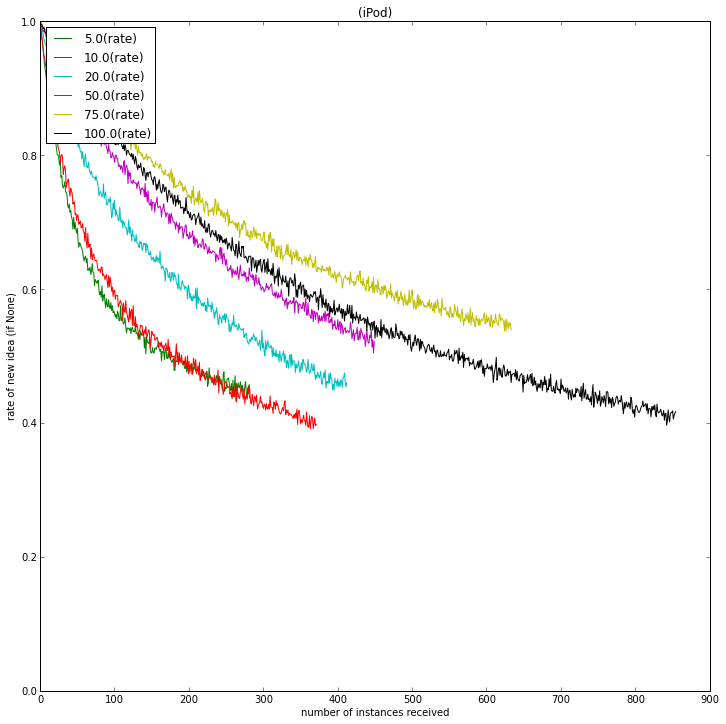
\includegraphics[width=0.7\columnwidth]{rate_new_idea_over_time}
    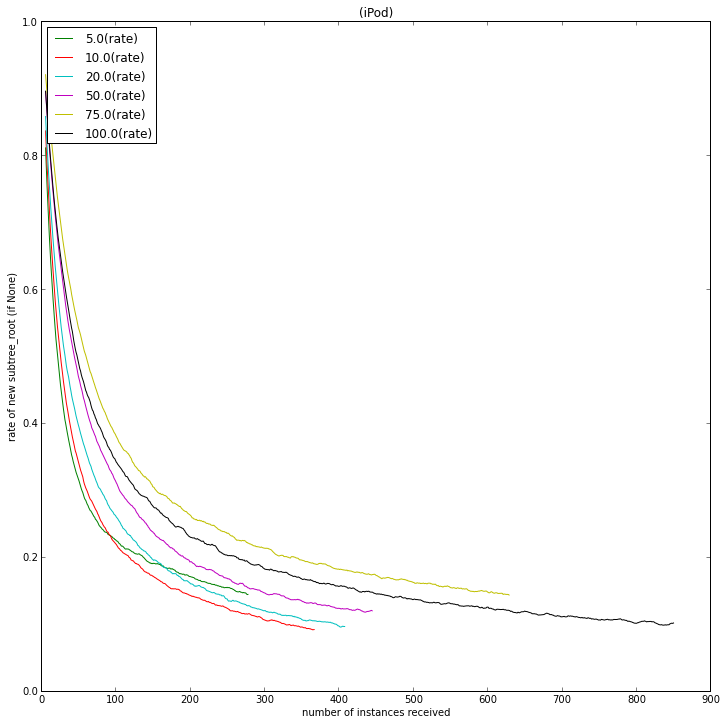
\includegraphics[width=0.7\columnwidth]{rate_new_category_over_time}
    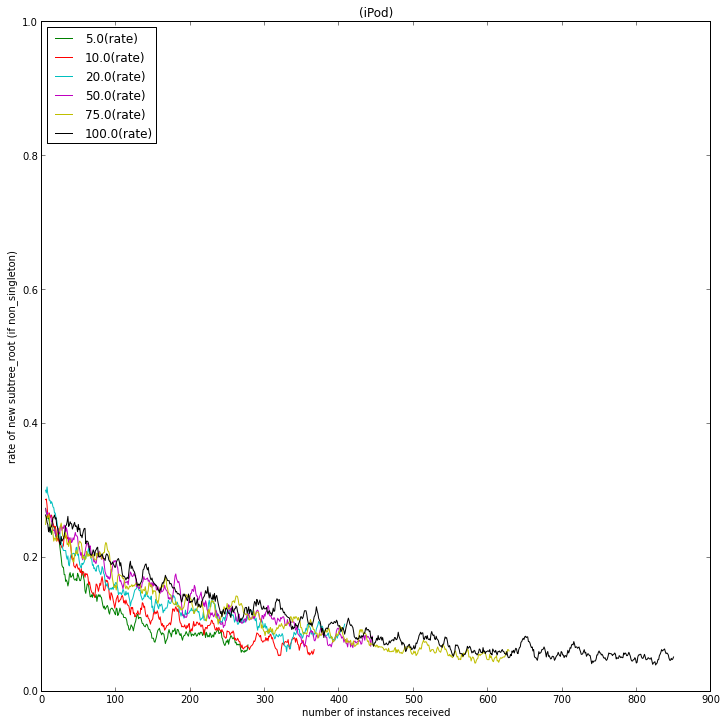
\includegraphics[width=0.7\columnwidth]{rate_new_ns_category_over_time}
    \caption{Rate of idea generation}
\end{figure}

The number of ideas, categories and non-singleton each drop off exponentially over time. It is unsurprising that the number of new categories should drop off faster than the number of new ideas, as we expect that there are fewer categories of ideas than there are individual ideas themselves.

The third panel, which shows non-singleton categories over time, tells a distinctly different story from the others. While in the idea and category plots, the height-ordering of rates of generation between categories remains generally identical, there is a point of intersection and reversal in the non-singleton category plot at around the 30 instances point. Before this point, the lower conditions actually generate new categories at a \emph{faster} rate.

In lower conditions, brainstormers will quickly offer up big, popular, non-singleton categories. Beyond the inflection point, the category pool is saturated with these low-hanging fruit, and only brainstormers tasked with generating more ideas will find the smaller category. This is a more nuanced view of the tree node/instance quartiles in Section SEC; condition 5 brainstormers cover the spectrum of category sizes while condition 100 brainstormers pull from the smaller category trees in the forest.

\subsubsection{Hypothesis 1}

Visually, the rate of idea, category and singleton category generation seems to trend towards 0. We tested this hypothesis...

Additionally Figure FIG indicates that there is some effect of number of ideas requested on the rate of generation. Generally, conditions with more requested responses generated ideas and categories at a higher rate.

Test here...

\subsubsection{Hypothesis 2}

Test here...

\subsection{Originality}

We measure differences in originality between conditions by examining the idea o-score and category o-score. The distributions of these scores are summarized in Figure FIG. The left panel compares idea o-score and the right compares category o-score.

\begin{figure}[h!]
    \centering
    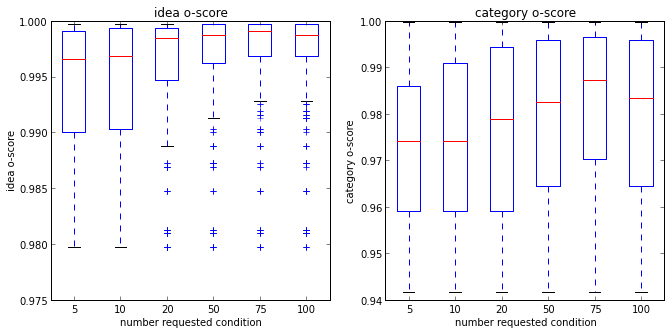
\includegraphics[width=0.9\columnwidth]{oscores_conditions}
\end{figure}

The more ideas requested, the more original the ideas produced. As suggested by the instance quartile range in section SEC, higher number conditions produce idea in trees with fewer instances, thus the high category o-score. We also see that these conditions produce \emph{ideas} with fewer instances.

As the originality rises, however, so does the number of outliers. To understand this phenomenon, we need to more closely observe the distribution of originality scores between not just conditions, but ordinal position in a brianstorming run.

Figure FIG provides this visualization. The upper panel gives the mean idea o-score as a function of ordinal position in all 100 condition brainstorming runs. The o-score for each ordinal position is the mean of all idea o-scores for that ordinal position in a run. Following this, the plot is further smoothed by making each point the mean of a sliding window of size 10 around its ordinal position. The bottom panel is a similar plot for category-oscore. To aid in interpretation, the first, second and third quartiles are also represented on the plot. The error bars are standard error.

\begin{figure}[h]
    \centering
    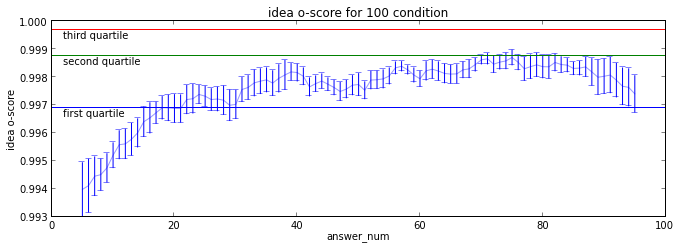
\includegraphics[width=0.9\columnwidth]{idea_oscore_order_100}
    \caption{Idea o-score as a function of order (100 condition)}
    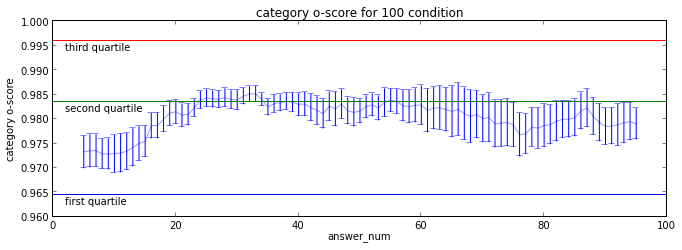
\includegraphics[width=0.9\columnwidth]{cat_oscore_order_100}
    \caption{Category o-score as a function of order (100 condition)}
\end{figure}

The only part of the originality score that falls outside the first and third quartiles is the beginning of the run. Participants in the higher numbered conditions generate more original ideas overall, but not until they have exceeded some threshold of common ideas. Figure FIG replicates figure FIG but across all conditions, and the same pattern of originality growth until an originality peak - around 20 ideas - is reached. Note that because of the additional HITs, there are far more examples of early-order ideas in the 5, 10 and 20 conditions than in the 50, 75, or 100, so this pattern is present without any dominating affect by the upper conditions.

\begin{figure}[h]
    \centering
    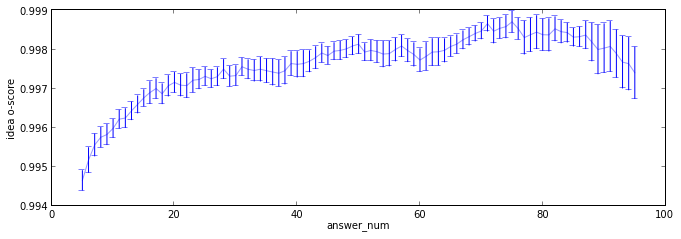
\includegraphics[width=0.9\columnwidth]{idea_oscore_order}
    \caption{Idea o-score as a function of order}
    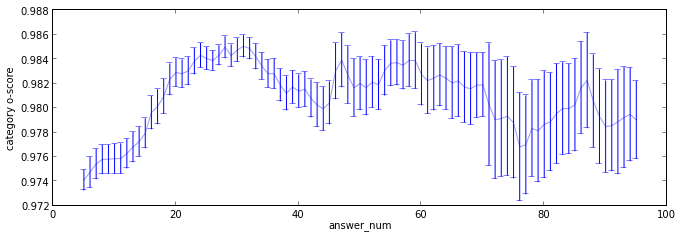
\includegraphics[width=0.9\columnwidth]{cat_oscore_order}
    \caption{Category o-score as a function of order}
\end{figure}

A similar, although less severe, pattern is observed for category o-score. There is a gradual increase in category originality until the 20 instance threshold is reached, at which point variance of the scores increases rapidly and no clear pattern is observable. This is explained by the relationship between common ideas and common categories. We expect that unoriginal ideas belong to unoriginal categories, as a high instance count for an idea increases the instance count for its category tree. However, we cannot make the inverse assumption, that a high originality idea belongs to a high originality category. Once the common idea are exhausted, then, there is no relationship between idea originality and category originality.

\subsubsection{Hypothesis 6}

This threshold at 20 ideas brings us to \textbf{Hypothesis 6:} Ideas generated in the latter half of a brainstorming session are of higher originality than ideas generated in the former half. With our empirical evidence, we can instead test that ideas \emph{more than 20 instances into a brainstorming session} are more original than those in the first 20 instances, regardless of condition.

Test here...

\subsection{Riffing: We need to change the name of this}

At the level of the individual brainstorming run, we examine a new phenomenon related to uniqueness above. Within the SIAM model, \emph{riffing} (or \emph{clustering} as it is known in the work) occurs when a single participant activates a single image (analogous to a non-singleton category) and produces multiple ideas from that image under a fail state is reached and a transition is undergone to a new image. Unsurprisingly, we observed riffing activity in our data. An example of a single participant's riffed responses is given in Figure FIG. The second column is dark if the instance is a \emph{look-back equal} to any idea earlier in the run. The first column is dark if the instance is a \emph{source} instance, meaning it is the first in a chain of look-back equal instances. Riff chains can either be consecutive (as in the example), or separated with instances in between. The third column simply provides the text for that instance.

\begin{figure}[h]
    \centering
    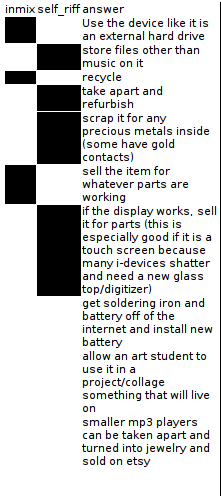
\includegraphics[width=0.5\columnwidth]{10_riff}
    \caption{Example of riffing in a size 10 run}
\end{figure}

The participant hits on the categories of using the device's hard drive for storage, recycling the device or its materials, and selling the device.  within these categories, they generate 2-3 ideas each. This is a fairly typical example of riffing. In larger conditions, it is common for participants to reach further back and return to an idea multiple time. Table TAB provides a summary of riffing between conditions.

\begin{table}
\begin{tabular}[h!]{r | l l l l l l l}
    \hline \hline \textbf{condition} & 5 & 10 & 20  \\ \hline \hline
    \% riffs & 13.65 & 19.28 & 25.17  \\
    source instances & 10.58 & 12.92 & 15.01 \\
    riffs per source & 1.29 & 1.49 & 1.68 \\
    median length of consecutive chain & 2 & 2 & 2 \\
    median distance to previous in chain & 1 & 2 & 2 \\
    median distance to first in chain & 2 & 3 & 5 \\ \hline \hline
    \textbf{condition} & 50 & 75 & 100 \\ \hline \hline
    \% riffs & 39.6 & 32.81 & 42.81 \\
    source instances & 19 & 17.19 & 18.13\\
    riffs per source & 2.08 & 1.91 & 2.36\\
    median length of consecutive chain & 2 & 2 & 2\\
    median distance to previous in chain & 7 & 10 & 5\\
    median distance to first in chain & 16.5 & 18 & 26.5 \\
    \end{tabular}
    \caption{Riffing statistics by condition}
\end{table}

The higher the number of instances requested, the more participants riff on their old ideas. Similarly, upper conditions use more of their ideas as sources for riffing, and riff more times on each of those ideas. The primary surprise is that they do not riff more consecutively. The median length of a consecutive riff chain remains low across conditions. This leaves us with the image of a participant in the upper conditions searching through their old ideas for something to build upon one instance at a time.

Another outlier of note is the relatively short median distance to a previous idea in a chain for the 100 condition. Participants in the 100 condition may feel more pressure to remix, and return to earlier ideas more quickly than those in the 50 or 75 conditions.

\subsubsection{Hypothesis 4}

Riffing activity is analogous to idea production within an image as described by Nijstad and Stroebe's SIAM model \cite{nijstad_how_2006}. Thus, we should expect to confirm their hypothesis, \textbf{Hypothesis 4}, that \emph{an idea from one semantic category should more often by followed by an idea from the same category than expected by random chance}.

To test this, we modelled the probability of any category being followed by the same category with a Bernoulli distribution. Each instance not the first in its run was a trial. If the instance was in the same category tree as the previous instance, the trial was a pass. Otherwise, it was a failure. The Bernoulli $\theta$ was 0.156 (95\% HDI 0.143 - 0.170).

The most common category tree in our data set, \emph{music player}, represents only 5.65\% of instances. This is well below the 0.143 lower-bound of HDI. Thus, we accept the hypothesis that an instance follows a previous instance in the same category with greater probability than is explained by random chance.

\subsection{Completion Time}

As another aspect of how participants complete brainstorming runs, we are interested in the time spent on each response. The first, second and third quartiles for each condition are given in boxplots in figure FIG. The whiskers extend to 1.5 times the inner quartile range. Surprisingly, we see many instances taking up to 28018382ms (7.78 hours) to complete.

\begin{figure}[h]
    \centering
    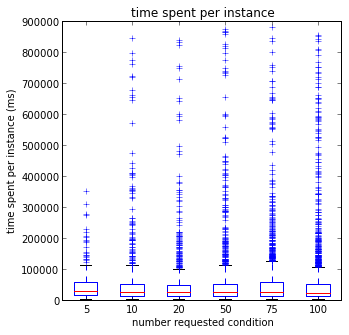
\includegraphics[width=0.9\columnwidth]{time_spent_condition}
    \caption{Time spent per instance}
\end{figure}

Either our participants were exceedingly concerned with crafting their responses, or there is another influence at work. Figure FIG gives the mean time spent on an instance by order, separated by condition. Most of the highly variant response times take place early in the brainstorming run. This suggests that at least one participant accepted a brainstorming task, took an initial stab at instances, and then left the task for up to 8 hours before continuing. Beyond this, we might expect to see time spent per instance go up as participants have to dig deeper to find responses, but no such effect is consistently observed.

\begin{figure}[h]
    \centering
    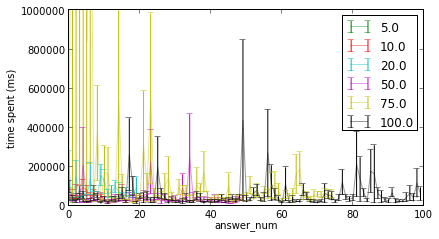
\includegraphics[width=0.9\columnwidth]{time_spent_order}
    \caption{Time spent per instance}
\end{figure}

\subsubsection{Hypotheses 5}

The Nijstad and Stroede \cite{nijstad_how_2006} model also provides \textbf{Hypothesis 5}: \emph{idea generation when changing semantic categories should take longer than idea generation within categories}. An examination of the distribution of data for time spent per instance suggested a log-normal distribution, with the frequency of occurances quickly rising until a peak was reached, followed by a gradual drop-off. As with previous tests, we used the Stan package for Bayesian inference [CITE]. We fit, two models: $t_w = \text{lognormal}(\mu_w, \sigma_w)$ for within-category idea generation and $t_b = \text{lognormal}(\mu_b, \sigma_b)$ for between-category idea generation, where the $t$ parameter in each model represents the time spent generating an instance.

\begin{figure}[h]
    \centering
    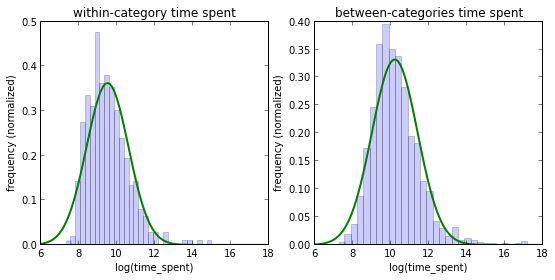
\includegraphics[width=0.9\columnwidth]{hyp5_comparison}
    \caption{Time spent to generate an instance}
\end{figure}

The resulting fit models are shown in Figure FIG, overlapping the log-space histograms for observed values. The mean for the within-category condition was 9.5 in log space (13.4 seconds, 95\% HDI 9.4-9.6), while the mean for the between-categories condition was 10.2 (27.0 seconds, 95\% HDI 10.2-10.3). The variances were 1.1 (3 seconds) and 1.2 (3.3 seconds) respectively. These difference were both sigificant. Within-category instance generation took on average 12.6 seconds less than between-categories. This is consistent with the findings of Nijstad and Stoebe, who reported differences of 6-12 seconds.
